%\def\dfdx#1#2{\frac{\partial {#1}}{\partial {#2}}}
%\begin{document}
%\newpage
\chapter{Multi body system model}
\label{chap:multi_mdl}
This chapter discusses two modelling approaches used in the Kalman filter.
% Multi body system 
In the first approach, the robot is modelled as multi body dynamic system in which the motion of the robot is caused by application of torques at the respective joints.
% sensor fusion
In the second approach a sensor fusion algorithm is implemented which depends on the motion equations developed from a simplified model of a inertial navigation system.
\section{Multi body system}
Humanoid robots consists of group of rigid bodies that are joined together to resemble the human skeletal structure. As human beings are driven by the muscular system, humanoids are driven by electric, hydraulic or pneumatic actuators, which apply torques at the joints of the robot. The dynamics of robots describes how the robots moves in response to the actuator forces or torques. The dynamics of the robot is defined by the  equations of motion of the rigid body system. In general there are several approaches in deriving equations of motion of rigid body dynamic system. One such approach is by deriving Lagrange equation. Lagrangian analysis relies on the energy properties of the mechanical system to derive the equations of motion. The \emph{Lagrangian, L,} is defined as the difference between kinetic and potential energy of the system. $$ L(q,\dot{q}) = T(q,\dot{q}) - V(q)$$ \emph{q} represents the vector of joint angles \emph{T} and \emph{V} represents the kinetic and potential energies of the system. \emph{q} is called the generalized coordinates of the system as the specification of joint angles uniquely determines position of all the rigid bodies.

The equations of motion for a rigid body system with generalized coordinates $q \in \Re^m $ is given by, 
\begin{align}
\frac{d}{dt} &\dfdx{L}{\dot{q}}-s\dfdx{L}{q_i} = \Gamma_i && i=1,....,m
\end{align}
$\Gamma_i$ is the external force acting on the $i^{th}$ generalized coordinate.
The general formulation of equation of motion of a multi body system is
\begin{equation}
\label{eq:dyn_mul_bdy}
M(q)\ddot{q}+C(q,\dot{q})+g(q) = \tau + \tau_{ext}
\end{equation}
\emph{M(q)} is the generalized inertia matrix, $C(q,\dot{q})$ is the matrix representing Coriolis and centrifugal forces, \emph{g(q)} is the gravity vector acting on the system and $\tau$ is the actuator torque applied to the joints $\tau_{ext}$ is the external torque acting on the system.
\begin{figure}
\begin{center}
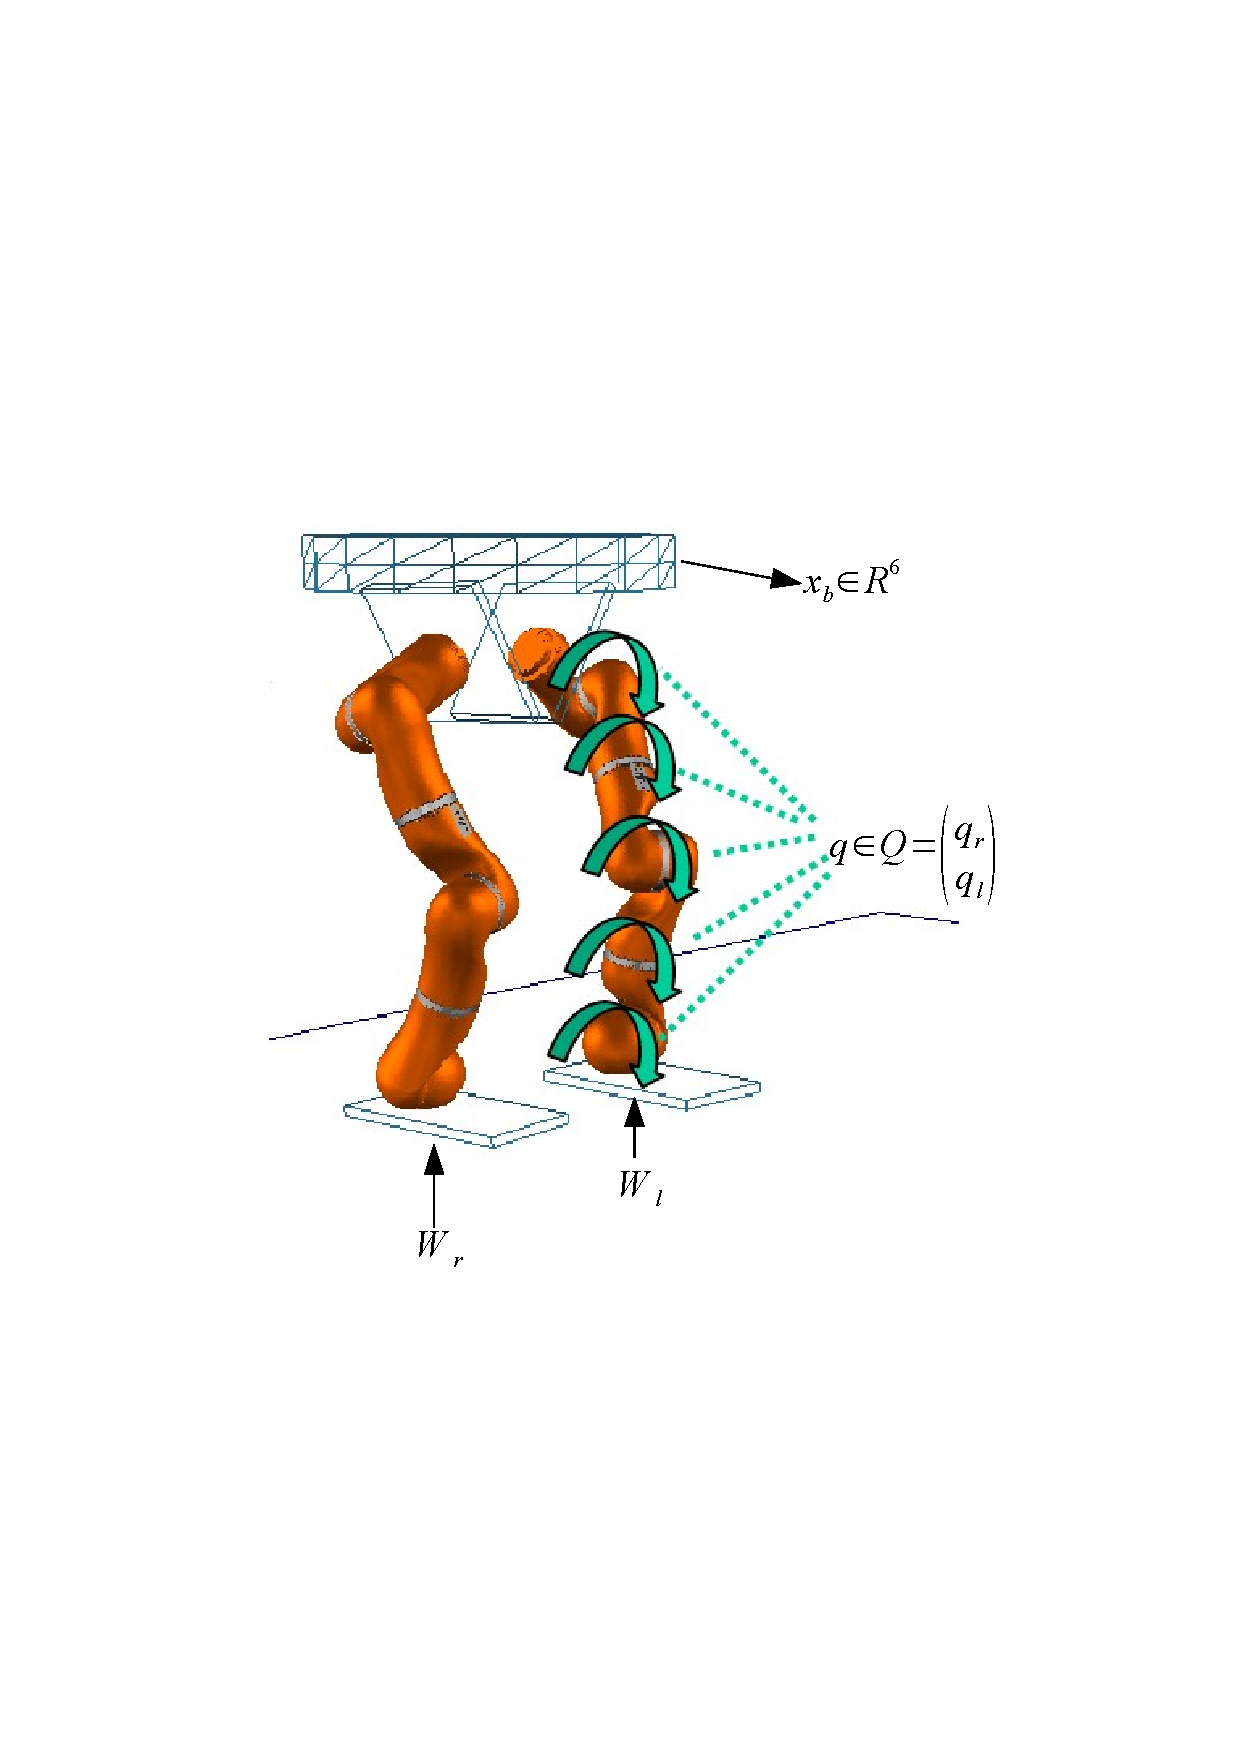
\includegraphics[trim= 10mm 80mm 10mm 80mm,scale=0.75]{Bilder/model_biped.pdf}
\caption{Simplified lower body model of biped}
\label{fig:biped_simplelow}
\end{center}
\end{figure}

Figure \ref{fig:biped_simplelow} shows a biped with two legs, which is connected to common base. $q$ represents a vector of joint variables which corresponds to angle of the joint. $q_r,q_l$ corresponds to joins in left and right legs respectively. Number of joints corresponds to the number of controllable degrees of freedom of the robot. \emph{Q} is the \underline{configuration space} of the biped. $x_b$ represents the number of degrees of freedom of the base. A rigid body in space has six degrees of freedom as shown in Figure \ref{fig:rbody} 
\begin{figure}[!htb]
\begin{center}
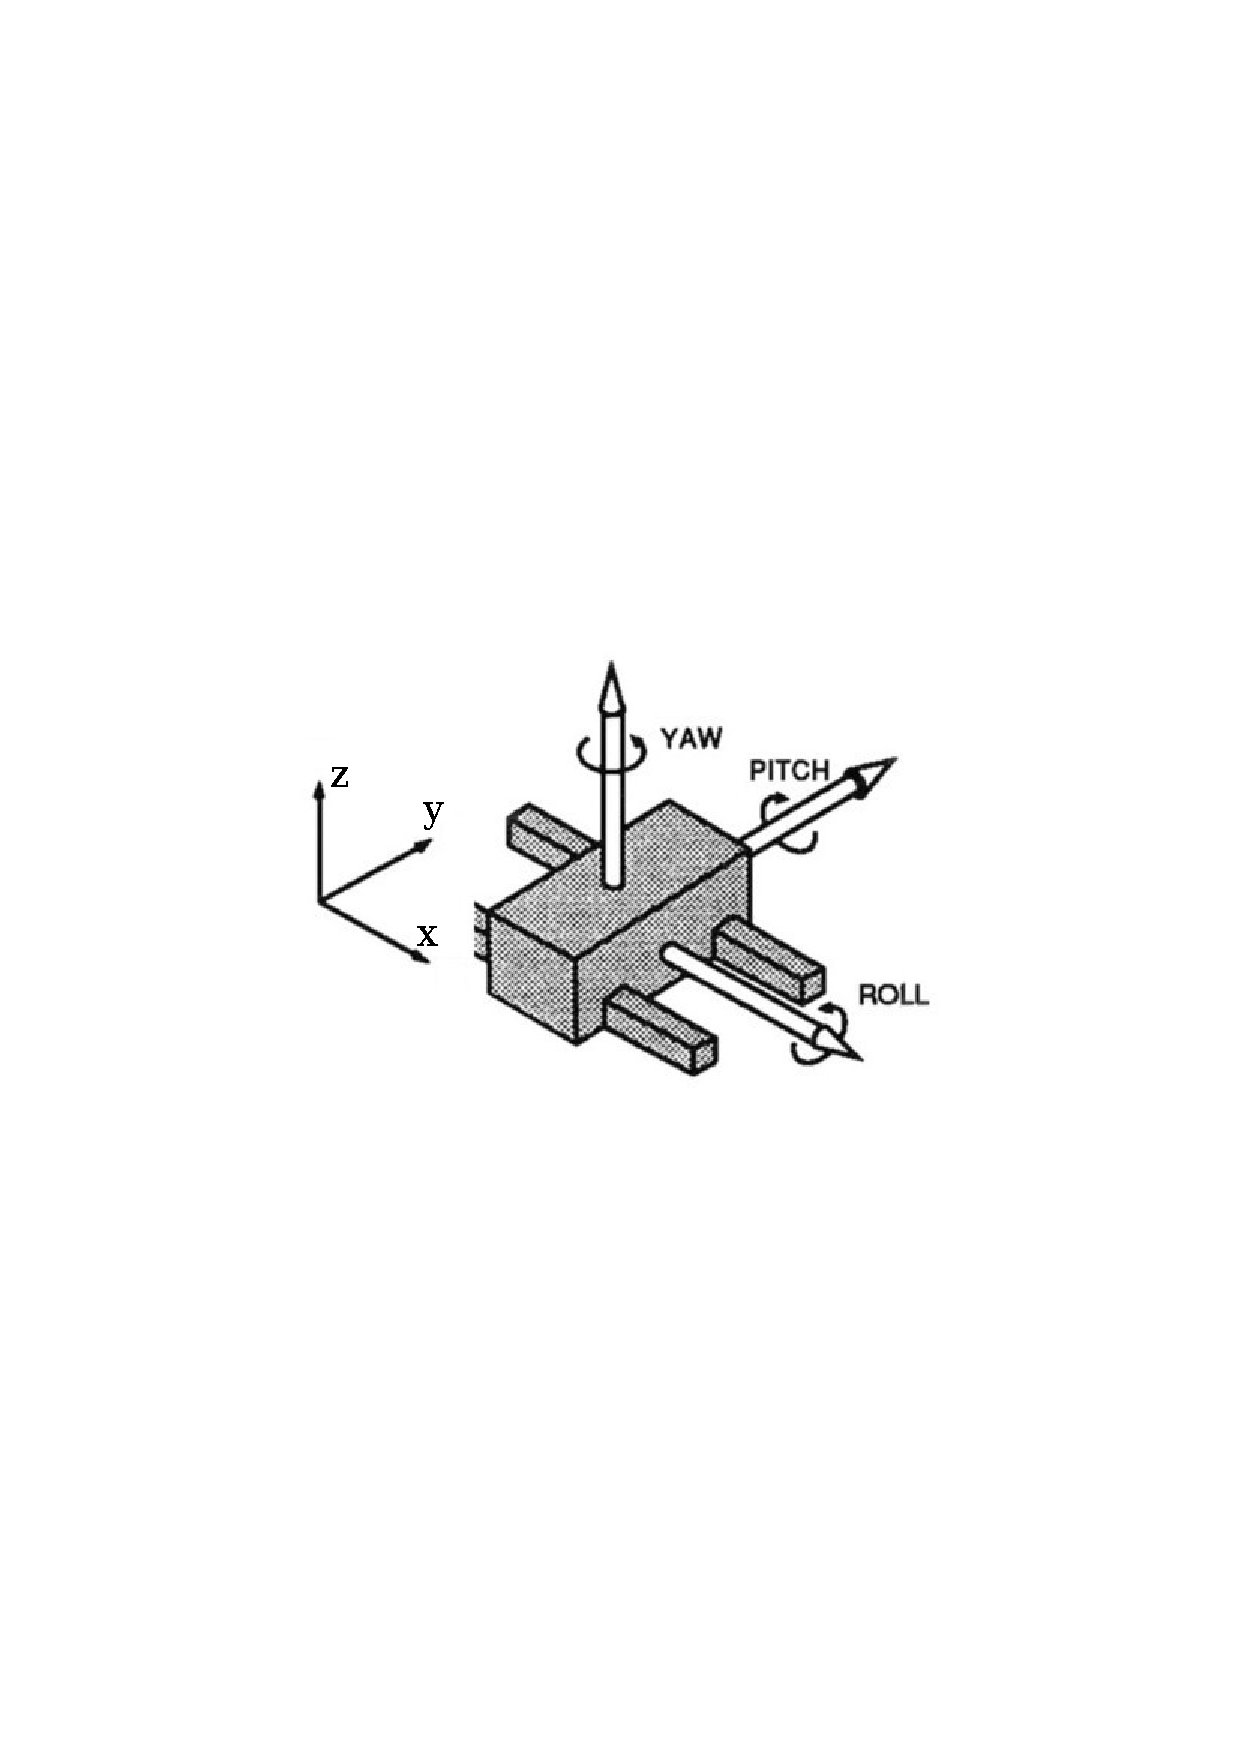
\includegraphics[trim= 10mm 100mm 10mm 120mm,scale=0.75]{Bilder/rbody_dof.pdf}
\caption[Degrees of freedom of a rigid body]{Degrees of freedom of a rigid body \footnotemark[1]}
\label{fig:rbody}
\end{center}
\end{figure}
where \emph{x,y,z} are the translational degrees of freedom and \emph{roll,pitch,yaw} are the rotational degrees of freedom which corresponds to rotation around \emph{x,y,z} axes respectively. In biped the base is a free rigid body which is unactuated. The base has all six degrees of freedom unless it is constrained to the surface as shown in Figure \ref{fig:biped_simplelow}. Since the base has all the six degrees of freedom it is called \emph{floating base} (i.e it is considered as floating in space). The equation of motion of the floating base is given by Newton-Euler equation of motion in body coordinates \citet[chapter 4]{mur94}.
\footnotetext[1]{Image source:\url{http://www.cncexpo.com/Images/pitchyawroll.jpg}}
\begin{equation}
\label{eq:dyn_rig_bdy}
\begin{bmatrix}
mI &0 \\ 0 &\Im
\end{bmatrix}
\begin{bmatrix}
\dot{v}^b\\ \dot{\omega}^b
\end{bmatrix}
+ \begin{bmatrix}
\omega^b \times mv^b \\ 
\omega^b \times \Im w^b
\end{bmatrix}
= W^b\\
\end{equation}
\emph{m} is the mass of the rigid body, $\Im$ is the inertia of the rigid body. $I,0$ are the $3 \times 3$ identity and zero matrices. $[\dot{v}^b,\dot{\omega}^b]$ are the \underline{body twist coordinates} of the rigid body. $W^b$ is the \underline{body wrench}  applied to the center of mass of body.
\begin{equation}
\label{eq:dyn_rig_bdy_sh}
M_x^b \ddot{x}_f^b + C_x^b\dot{x}_f^b+g_x^b = W^b
<<<<<<< HEAD
\end{equation}
To be consistent with the multi body system dynamics formulation in Equation \ref{eq:dyn_mul_bdy} Newton Euler Equation \ref{eq:dyn_rig_bdy} is reformulated into Equation \ref{eq:dyn_rig_bdy_sh}. $x_f^b$ is a vector that represents six degrees of freedom of the rigid body. $\dot{x}_f^b$ represents the body twist. $\ddot{x}_f^b$ represents the acceleration in body frame(i.e it represents the time derivative of body twist). $M_x^b$ represents the inertia matrix of the rigid body in body coordinates. $C_x^b$ is the matrix representing the Coriolis and centrifugal forces acting on the system in body coordinates. $g_x^b$ is the vector representing the gravitational forces acting on the body in body coordinates. $W^b$ is the external force applied to the center of mass of the body. \footnote[2]{Inertia, Coriolis and gravity are assumed to be given with respect to the body coordinate frame for the rest of the report}.

The dynamics of biped in Figure \ref{fig:biped_simplelow} is composed of both multi body dynamics in the form of legs and rigid body dynamics in form of base. Combining Equation \ref{eq:dyn_rig_bdy_sh} and Equation \ref{eq:dyn_mul_bdy} gives the equation of the biped.
\begin{equation} \label{eq:dyn_biped}
\begin{bmatrix}
M_x &M_{xq} \\ M_{qx} &M_q
\end{bmatrix}
\begin{bmatrix}
\ddot{x}_f \\ \ddot{q}
\end{bmatrix}
+
\begin{bmatrix}
C_x &C_{xq} \\ C_{qx} &C_q
\end{bmatrix}
\begin{bmatrix}
\dot{x}_f \\ \dot{q}
\end{bmatrix}
+
\begin{bmatrix}
g_x \\ g_q
\end{bmatrix}
=
\begin{bmatrix}
0 \\ \tau
\end{bmatrix}
+ (J_r^b)^T W_r^b + (J_l^b)^T W_l^b
\end{equation}
\underline{Explanation of the terms in the equation are part of appendix}.
Equation \ref{eq:dyn_biped} can be written in a simplified form as
\begin{equation} \label{eq:dyn_sbiped}
M(y)\ddot{y} + C(y,\dot{y})\dot{y} + g(y) = W_{act} + W_{ext}
\end{equation}
where $y = [x_f,q]^T$ is the combined state variables of the biped. $M(y),C(y),g(y)$ are combined Inertia, Coriolis and gravity parameters of the biped.
\begin{figure}
\begin{center}
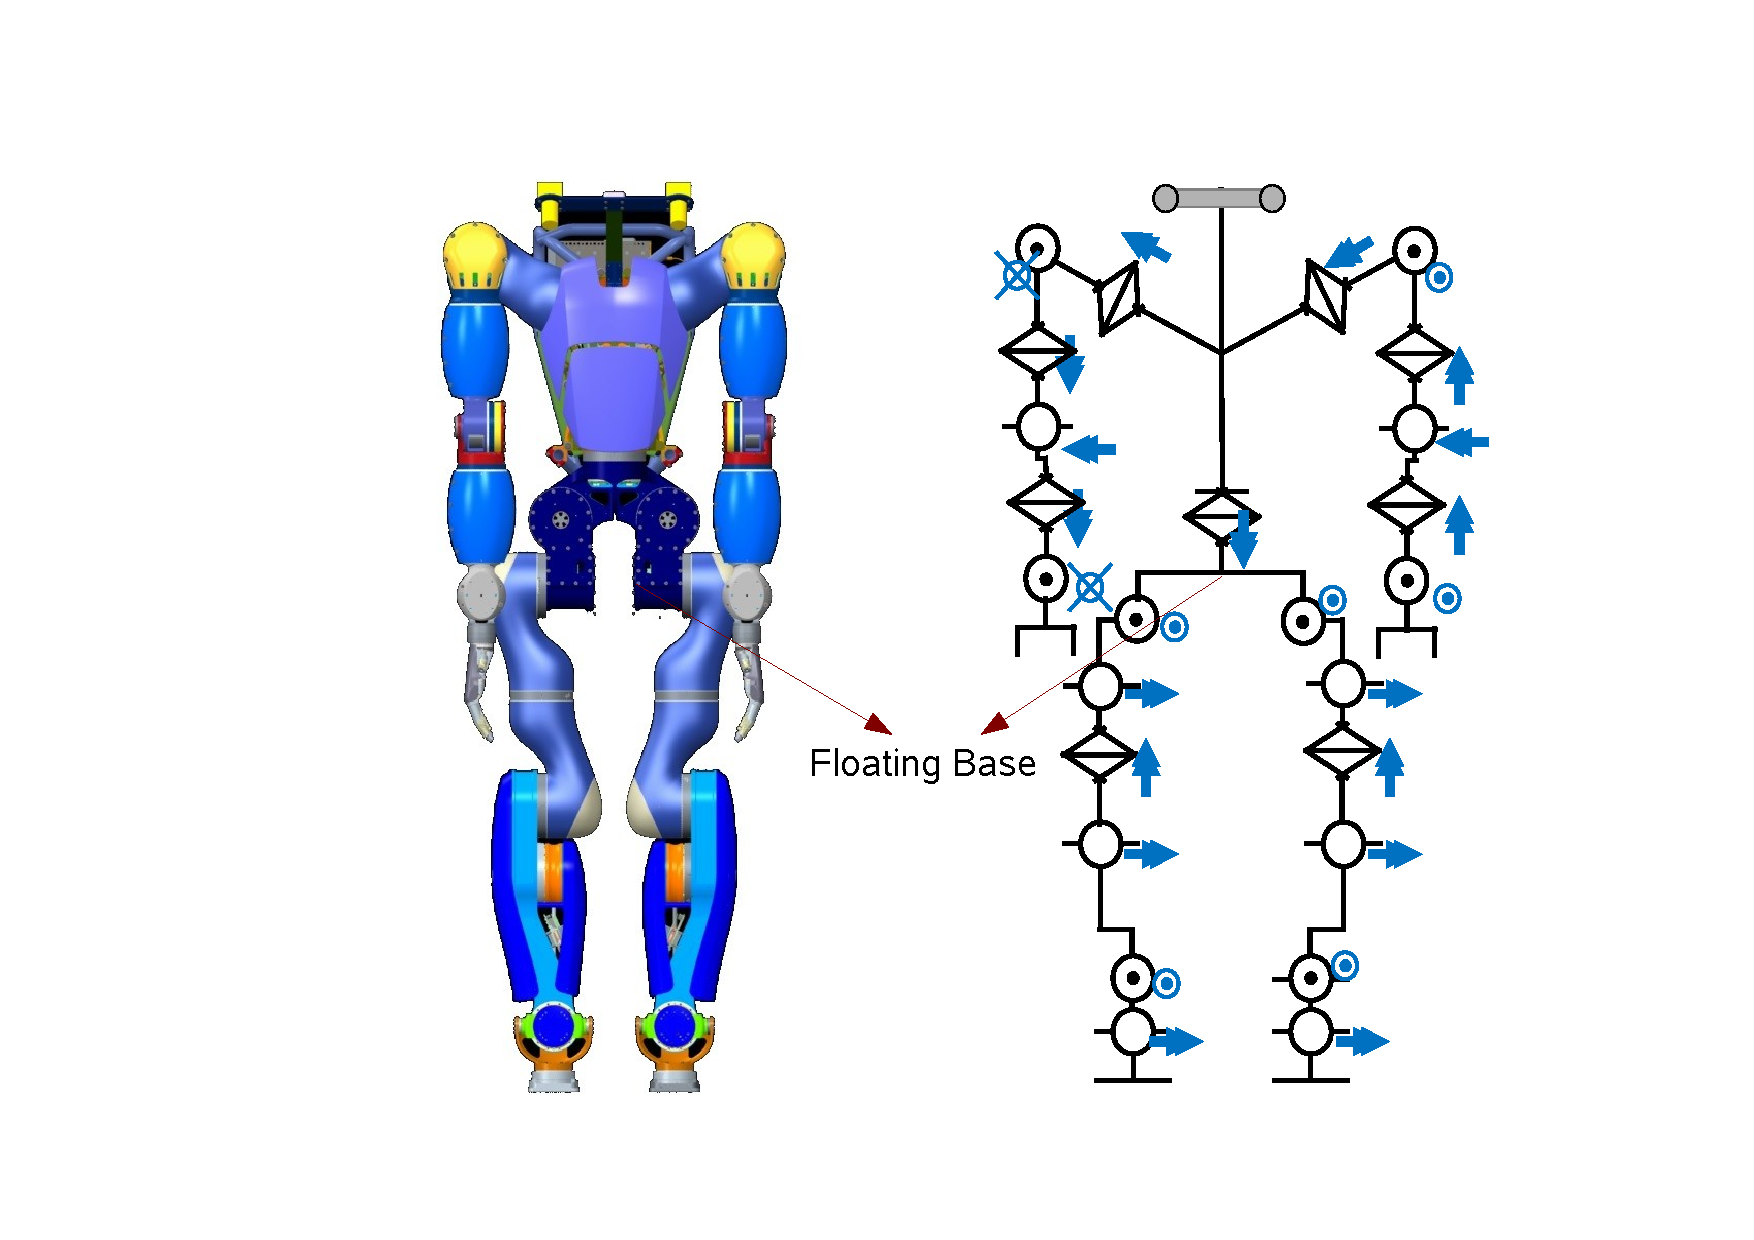
\includegraphics[trim= 70mm 10mm 40mm 10mm,clip,scale=0.7]{Bilder/TORO_kinematic.pdf}
\caption{Kinematic chain of \emph{Toro} \underline{Explain the joints symbols}}
\label{fig:toro_kin}
\end{center}
\end{figure}

=======
\end{equation}
To be consistent with the multi body system dynamics formulation in Equation \ref{eq:dyn_mul_bdy} Newton Euler Equation \ref{eq:dyn_rig_bdy} is reformulated into Equation \ref{eq:dyn_rig_bdy_sh}. $x_f^b$ is a vector that represents six degrees of freedom of the rigid body. $\dot{x}_f^b$ represents the body twist. $\ddot{x}_f^b$ represents the acceleration in body frame(i.e it represents the time derivative of body twist). $M_x^b$ represents the inertia matrix of the rigid body in body coordinates. $C_x^b$ is the matrix representing the Coriolis and centrifugal forces acting on the system in body coordinates. $g_x^b$ is the vector representing the gravitational forces acting on the body in body coordinates. $W^b$ is the external force applied to the center of mass of the body. \footnote[2]{Inertia, Coriolis and gravity are assumed to be given with respect to the body coordinate frame for the rest of the report}.

The dynamics of biped in Figure \ref{fig:biped_simplelow} is composed of both multi body dynamics in the form of legs and rigid body dynamics in form of base. Combining Equation \ref{eq:dyn_rig_bdy_sh} and Equation \ref{eq:dyn_mul_bdy} gives the equation of the biped.
\begin{equation} \label{eq:dyn_biped}
\begin{bmatrix}
M_x &M_{xq} \\ M_{qx} &M_q
\end{bmatrix}
\begin{bmatrix}
\ddot{x}_f \\ \ddot{q}
\end{bmatrix}
+
\begin{bmatrix}
C_x &C_{xq} \\ C_{qx} &C_q
\end{bmatrix}
\begin{bmatrix}
\dot{x}_f \\ \dot{q}
\end{bmatrix}
+
\begin{bmatrix}
g_x \\ g_q
\end{bmatrix}
=
\begin{bmatrix}
0 \\ \tau
\end{bmatrix}
+ (J_r^b)^T W_r^b + (J_l^b)^T W_l^b
\end{equation}
\underline{Explanation of the terms in the equation are part of appendix}.
Equation \ref{eq:dyn_biped} can be written in a simplified form as
\begin{equation} \label{eq:dyn_sbiped}
M(y)\ddot{y} + C(y,\dot{y})\dot{y} + g(y) = W_{act} + W_{ext}
\end{equation}
where $y = [x_f,q]^T$ is the combined state variables of the biped. $M(y),C(y),g(y)$ are combined Inertia, Coriolis and gravity parameters of the biped.
\begin{figure}
\begin{center}
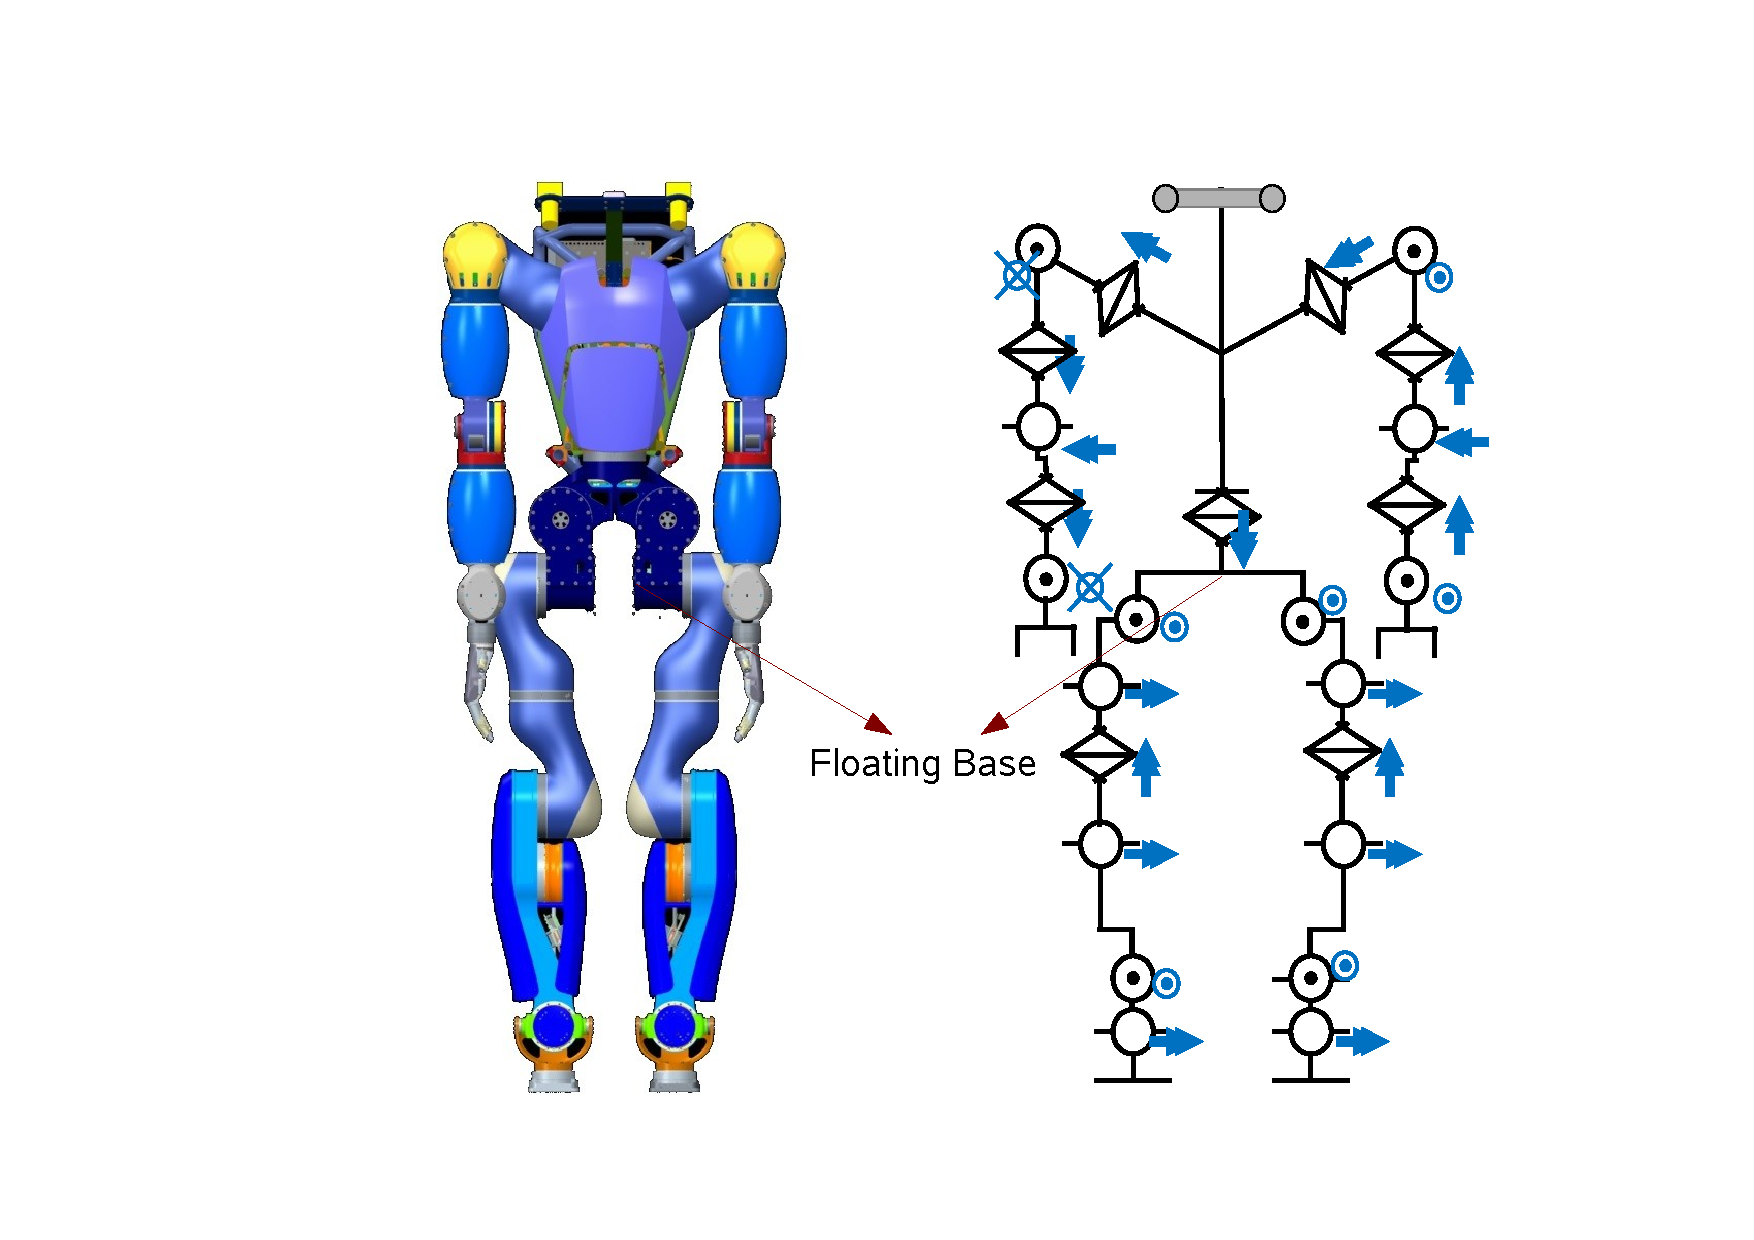
\includegraphics[trim= 70mm 10mm 40mm 10mm,clip,scale=0.7]{Bilder/TORO_kinematic.pdf}
\caption{Kinematic chain of \emph{Toro} \underline{Explain the joints symbols}}
\label{fig:toro_kin}
\end{center}
\end{figure}

>>>>>>> 44a31b53d04194cb885ea2522465b774c238d9f2
\emph{Toro} is modelled as floating base dynamic model. \emph{Toro} is made up of 25 rotary joints that are actuated by electrical motors. It can be seen from Figure \ref{fig:toro_kin} that floating base acts as the root of the kinematic chain. Legs and torso branches out of the floating base. Equation of motion for \emph{Toro} can be formulated in similar fashion as biped Equation \ref{eq:dyn_sbiped}, where the dynamics of the upper body is also combined to it. The forward dynamics of \emph{Toro} 
\begin{equation}
	\label{eq:motion}
	\begin{split}
	\ddot{y} = M(y)^{-1}(&-C(y,\dot{y})\dot{y} - g(y) + J_r(y)^{T}W_{r} +J_l(y)^{T}W_{l} + \tau) \\
	\text{where,}\\ y &=
	\begin{bmatrix}
	 x_f \\ q 
	\end{bmatrix} \in \Re ^{31} \\
	x_f &= [p,\theta]^T \in \Re ^6 \\
	q &= [q_{1},q_{2},\ldots , q_{25}]^T \in \Re ^{25}\\
	\end{split}
\end{equation}
\emph{q} is a vector of joint variables given in generalized coordinates. $x_{f}=[p,\theta]^{T}$ is a vector of position and orientation defined with respect to spatial frame. $p=[p_x,p_y,p_z]$ is a vector representing  the position of origin of floating base with respect to spatial frame and $\theta=[\theta_{x},\theta_{y},\theta_{z}]$ is a vector of \underline{Euler angles}  that describes the rotation of floating base frame with respect to spatial frame. $q \in \Re^{25}$ is the vector of joint angles. $\dot{y}=[V^{b},\dot{q}]^T \in \Re^{31}$ is the vector of generalized velocities. $V^b= [v^b,\omega^b]^T \in \Re^{6}$ is the body velocity, it is defined in \ref{eq:body_vel}. $\dot{q} \in \Re^{25}$ is the vector of joint velocities. $\ddot{y}\in \Re^{31}$ is the vector of generalized accelerations. $M(y)\in \Re^{31 \times 31}$ is the inertia matrix, $C(y,\dot{y})\in \Re^{31 \times 31}$ is the matrix accounting for centrifugal and Coriolis forces. $g(y) \in \Re^{31}$ is the gravity vector. $\tau \in \Re^{31}$ is the vector of actuating torques acting on the robot, where the first six components are zero because those degrees of freedom corresponding to $x_f$ are not actuated. $J_r(y)^{T},J_l(y)^{T} \in \Re^{31 \times 6}$ represents the body Jacobian that transforms the wrenches $W_r,W_l \in \Re^{6}$ applied in the right and left foot to generalized forces acting on the robot.

Integrating the forward dynamics Equation \ref{eq:motion} once gives the velocity of all the bodies in the system and integrating it twice gives the position or orientation of the system. $$ acc = \dfdx{^2pos}{t}, vel = \dfdx{pos}{t} $$ 
\subsection{Space representation:}
The multi body system would be modeled with position(\emph{pos}) and velocity(\emph{vel}) as the state variables which leads to following form 
\begin{equation}
\label{eq:newton_motion}
 \begin{bmatrix}
\dot{pos} \\ \dot{vel}
\end{bmatrix}
= \begin{bmatrix}
vel \\ acc
\end{bmatrix}
\end{equation}
acceleration(\emph{acc}) is given by the forward dynamics of the system.

The equations of motion in Equation \ref{eq:motion} should be formulated in state space form of non linear systems as given in \ref{eqn:nl_sys}.
\begin{comment}
General state space representation of a non linear system
\begin{equation}
\label{eq:dyn_nl}
	\begin{split}
	\dot{x} = f(x,u)\\
	y = h(x,u)
	\end{split}
\end{equation}
where, $x \in \Re^{n}$ is the vector representing the states of the system. $u \in \Re^{p}$ is the vector of inputs acting on the system. $y \in \Re^{m}$ is the vector of outputs of the system.\\
\end{comment}
The velocity of the free floating base of the robot is modelled as body velocity $V_f^b$ which is given as,
\begin{equation}
\label{eq:body_vel}
V^b =
\begin{bmatrix}
v^b \\ \omega^b
\end{bmatrix}
= \begin{bmatrix}
R^T \dot{p} \\ (R^T \dot{R})^\vee
\end{bmatrix}
\end{equation}
$\vee$ operator denotes represents the extraction of 3 dimensional vector from the symmetric matrix[Appendix \ref{sec:avel_trfm}]
$\dot{p}$ is the time rate of change of the position of the body. \emph{R} is the rotation matrix which describes the rotation of rigid body with respect to \underline{spatial frame}. It is possible to reformulate the translational velocity of the above equation in first order \underline{ODE(Ordinary Differential Equation)}. It is not straight forward to obtain the time rate of change of Euler angles $\dot{\theta}$. There exists a transformation between the $\dot{\theta}$ and angular velocity $\omega^b$.
\begin{equation}
\label{eq:transfo_angvel}
\begin{split}
\omega^b = T(\theta)\dot{\theta}
\end{split}
\end{equation}
$T(\theta)$ is the transformation matrix [Appendix \ref{sec:avel_trfm}]. 

The state space representation of the equation of motions of \emph{Toro} can be obtained by substituting Equations \ref{eq:body_vel}, \ref{eq:transfo_angvel} and \ref{eq:motion} in Equation \ref{eq:newton_motion}

\begin{equation}
\label{eq:toro}
	\dot{x} = 
	\begin{bmatrix}
	\dot{p} \\ \dot{\theta} \\ \dot{q} \\ \ddot{y}
	\end{bmatrix}
	=
	\begin{bmatrix}
	R v^b\\	
	T(\theta)^{-1} \omega_f^b \\
	\dot{q}\\
	M(y)^{-1}(-C(y,\dot{y})\dot{y} -g(y) +  J_r(y)^{T}W_{r} +J_l(y)^{T}W_{l} + \tau)	
	\end{bmatrix}
	\\
	\end{equation}
	

\begin{itemize}
\item $$ y = \begin{bmatrix} p \\ \theta \\ q \end{bmatrix} = \begin{bmatrix} x_f \\ q \end{bmatrix}, \dot{y} = \begin{bmatrix} V^b \\ \dot{q}\end{bmatrix}, x = \begin{bmatrix}y \\ \dot{y}\end{bmatrix} $$  $x_f,q$ are the parameters of the floating base and joints as described in \ref{eq:motion}. $V^b$ is the body velocity as defined in \ref{eq:body_vel} and $\dot{q}$ is the velocities of the joints of the robot. \emph{x} is the vector of system states.
\item $T(\theta_{f})$ is the matrix that transforms the angular velocity $\omega_{f}^{b}$ to the time derivative of Euler angles $\dot{\theta}_{f}$. i.e $\omega_{f}^{b}=T(\theta_{f}) \dot{\theta}_{f}$. 
\item R is the rotation matrix which describes the rotation of floating base with respect to spatial frame. $ R = R_x(\theta_x) R_y(\theta_y) R_z(\theta_z)$
\end{itemize}

\section{Prediction Step}
The prediction equations of EKF are given in Equation \ref{eq:ekf_predict}. For the sake of simplicity we assume the process noise acting on the model is uncorrelated. i.e The noise acting on each state is independent $$W_k = I_{3}$$. Substituting the value of $W_k$ in Equation \ref{eq:ekf_predict}
\begin{equation}
\label{eq:predict}
\begin{split}
\hat{x}_{k+1}^- &= f(\hat{x}_{k},u_{k+1},0)\\
P_{k+1}^- &= A_kP_{k}A_k^T + Q_{k}\\
\end{split}
\end{equation}
The model is discretized for the implementation of EKF. Since the time step for integration is very small $\Delta t = 1ms$ forward Euler discretization method is used to discretize the continuous time model in \ref{eq:toro}.
\begin{equation}
\label{eq:toro_dis}
	\begin{bmatrix}
<<<<<<< HEAD
	\hat{p}_{k+1}^- \\ \hat{\theta}_{k+1}^- \\ \hat{q}_{k+1}^- \\ \hat{\dot{y}}_{k+1}^-
	\end{bmatrix}
	 =   
	 \begin{bmatrix}
	 \hat{p}_k \\ \hat{\theta}_k \\ \hat{q}_k \\ \hat{\dot{y}}_{k}
	\end{bmatrix}	  
	+ \Delta t f(\hat{x}_k,u_{k+1}) \\
\end{equation}
$$ f(\hat{x}_k,u_{k+1}) = 
	\begin{bmatrix}
	R v^b_k\\	
	T(\hat{\theta}_k)^{-1} \omega_k^b\\
	\dot{q_k}\\
	M(\hat{y}_{k})^{-1}(-C(\hat{y}_{k},\hat{\dot{y}}_{k})\hat{\dot{y}}_{k} -g(\hat{y}_{k}) +  J_r(\hat{y}_{k})^{T}W_{r,k+1} +J_l(\hat{y}_{k})^{T}W_{l,k+1} + \tau_{k+1})	
	\end{bmatrix} $$
$\hat{x}(t_k) = \hat{x}(k \Delta t) = \hat{x}_k$ represents the state x at \emph{kth} sampling instant. $\hat{x}_{k+1} = \hat{x}(k \Delta t + \Delta t)$ represents the state of the system at the next sampling instant. $u_{k+1}$ is the input at sampling instant $k+1$. It is assumed that the value of the input remains constant in the interval between two sampling instant. This assumption is valid because of the zero order hold mechanism in sensor circuitry.
=======
	p_{k+1} \\ \theta_{k+1} \\ q_{k+1} \\ \dot{y}_{k+1}
	\end{bmatrix}
	 =   
	 \begin{bmatrix}
	 p_{k} \\ \theta_{k} \\ q_{k} \\ \dot{y}_{k}
	\end{bmatrix}	  
	+ \Delta t f(x_k,u_{k+1}) \\
\end{equation}
$$ f(x_k,u_{k+1}) = 
	\begin{bmatrix}
	R v^b_k\\	
	T(\theta_k)^{-1} \omega_k^b\\
	\dot{q_k}\\
	M(y_k)^{-1}(-C(y_k,\dot{y}_k)\dot{y}_k -g(y_k) +  J_r(y_k)^{T}W_{r,k+1} +J_l(y_k)^{T}W_{l,k+1} + \tau_{k+1})	
	\end{bmatrix} $$
$x(t_k) = x(k \Delta t) = x_k$ represents the state x at \emph{kth} sampling instant. $x_{k+1} = x(k \Delta t + \Delta t)$ represents the state of the system at the next sampling instant. $u_{k+1}$ is the input at sampling instant $k+1$. It is assumed that the value of the input remains constant in the interval between two sampling instant. This assumption is valid because of the zero order hold mechanism in sensor circuitry.
>>>>>>> 44a31b53d04194cb885ea2522465b774c238d9f2

Equation \ref{eq:toro_dis} is used to predict the state $\hat{x}_k$ in Equation \ref{eq:predict}. For the computation of state covariance matrix $P_k^-$ in Equation \ref{eq:predict}, the \underline{Jacobian Matrix} is computed for Equation \ref{eq:toro_dis}. \underline{The Jacobian} computation of the different parts of the equation is follows,
From Equation \ref{eq:toro_dis}
\begin{enumerate}
<<<<<<< HEAD
\item $ \hat{p}_{k+1}^- = \hat{p}_k + \Delta t Rv_b$, $ \hat{p}_k = [\hat{p}_{x,k},\hat{p}_{y,k},\hat{p}_{z,k}]$
\begin{equation}
\label{eq:dpdx}
\dfdx{\hat{p}_{j,k+1}^-}{x} = \left(\dfdx{\hat{p}_{j,k+1}^-}{x_{1}}, \dfdx{\hat{p}_{j,k+1}^-}{x_{2}}, \cdots , \dfdx{\hat{p}_{j,k+1}^-}{x_{62}}\right) \in \Re^{3 \times 62}
\end{equation}
\[
 \dfdx{\hat{p}_{k+1}^-}{x_{i}} =  \left\lbrace
  \!\begin{aligned}
   &e_i & \text{if }(i=j)\\
   &\Delta t \dfdx{R}{x_i}v_b & \text{if }(3 < i \leq 6)\\
   &\textbf{0}_{3 \times 1} &\text{if}(6 < i \leq 31) \text{ or } (35 < i \leq 62) \\
   &col(R,i-31) & \text{if } 31 < i \leq 34 \\
=======
\item $ p_{k+1} = p_k + \Delta t Rv_b$, $ p = [p_x,p_y,p_z]$
\begin{equation}
\label{eq:dpdx}
\dfdx{p_{j,k+1}}{x} = \left(\dfdx{p_{j,k+1}}{x_{1}}, \dfdx{p_{j,k+1}}{x_{2}}, \cdots , \dfdx{p_{j,k+1}}{x_{62}}\right) \in \Re^{3 \times 62}
\end{equation}
\[
 \dfdx{p_{k+1}}{x_{i}} =  \left\lbrace
  \!\begin{aligned}
   &e_i & \text{if }(i=j)\\
   &\Delta t \dfdx{R}{x_i}v_b & \text{if }(3 > i \leq 6)\\
   &\textbf{0}_{3 \times 1} &\text{if}(6 > i \leq 31) \text{ or } (35 > i \leq 62) \\
   &col(R,i-31) & \text{if } 31 > i \leq 34 \\
>>>>>>> 44a31b53d04194cb885ea2522465b774c238d9f2
  \end{aligned} \right.
\]
\begin{itemize}
\item \emph{j} in the subscript represents the row dimension and  \emph{i} represents the column dimension of the matrix in Equation \ref{eq:dpdx}
\item $col(X,i)$ - represents the \emph{ith} column of matrix $X$.
<<<<<<< HEAD
\item $\dfdx{R}{x_i}$ is the partial derivative of \emph{R} with respect to the state $\hat{x}_k$ (i.e euler angles [Appendix \ref{sec:rot_mat}]), $e_i$ is the unit vectors in direction of coordinate axis and  $\textbf{0}_{3 \times 1}$ is the zero vector of dimensions $3 \times 1$ [Appendix \ref{sec:symbols}].
\end{itemize}

\item $\hat{\theta}_{k+1}^- = \hat{\theta}_k + \Delta t T(\hat{\theta}_k)^{-1} \omega_k^b$
\begin{equation}
\label{eq:dthetadx}
\dfdx{\hat{\theta}_{j,k+1}^-}{x} = \left(\dfdx{\hat{\theta}_{j,k+1}^-}{x_{1}}, \dfdx{\hat{\theta}_{j,k+1}^-}{x_{2}}, \cdots , \dfdx{\hat{\theta}_{j,k+1}^-}{x_{62}}\right) \in \Re^{3 \times 62}
\end{equation}
\[
 \dfdx{\hat{\theta}_{k+1}^-}{x_{i}} = \left\lbrace
  \!\begin{aligned}
   &\textbf{0}_{3 \times 1} &\text{if}(0 < i \leq 3) \text{ or }(6 < i \leq 31) \text{ or } (35 < i \leq 62) \\
   &e_{i-3} + \Delta t \dfdx{T(\hat{\theta}_k^-)^{-1}}{x_i}\omega_k^b & \text{if}3< \text{i} \leq 6 \\
   &col(T(\hat{\theta}_k^-)^{-1},i-34) & \text{if } 31 < i \leq 34 \\
  \end{aligned} \right.
\]
\begin{itemize}
\item $\dfdx{T(\theta_k^-)^{-1}}{x_i}$ is the partial derivative of inverse of transformation matrix with respect to state [Appendix \ref{sec:avel_trfm}] 
\end{itemize}

\item $\hat{q}_{k+1}^- = \hat{q}_k + \Delta t \dot{q}_k $
\begin{equation}
\label{eq:dqdx}
\dfdx{\hat{q}_{k+1}^-}{x} = \left(\dfdx{\hat{q}_{k+1}^-}{x_{1}}, \dfdx{\hat{q}_{k+1}^-}{x_{2}}, \cdots , \dfdx{\hat{q}_{k+1}^-}{x_{62}}\right) \in \Re^{25 \times 62}
\end{equation}
\[
\dfdx{\hat{q}_{k+1}^-}{x_{i}} = 
	\begin{cases}
	l_{25,i} & \text{if } (6 < i \leq 31) \text{ or } (38 < i \leq 62) \\
=======
\item $\dfdx{R}{x_i}$ is the partial derivative of \emph{R} with respect to the state $x_k$ (i.e euler angles [Appendix \ref{sec:rot_mat}]), $e_i$ is the unit vectors in direction of coordinate axis and  $\textbf{0}_{3 \times 1}$ is the zero vector of dimensions $3 \times 1$[Appendix \ref{sec:symbols}].
\end{itemize}

\item $\theta_{k+1} = \theta_k + \Delta t T(\theta_k)^{-1} \omega_k^b$
\begin{equation}
\label{eq:dthetadx}
\dfdx{\theta_{j,k+1}}{x} = \left(\dfdx{\theta_{j,k+1}}{x_{1}}, \dfdx{\theta_{j,k+1}}{x_{2}}, \cdots , \dfdx{\theta_{j,k+1}}{x_{62}}\right) \in \Re^{3 \times 62}
\end{equation}
\[
 \dfdx{\theta_{k+1}}{x_{i}} = \left\lbrace
  \!\begin{aligned}
   &\textbf{0}_{3 \times 1} &\text{if}(0 > i \leq 3) \text{ or }(6 > i \leq 31) \text{ or } (35 > i \leq 62) \\
   &e_{i-3} + \Delta t \dfdx{T(\theta_k)^{-1}}{x_i}\omega_k^b & \text{if}3> \text{i} \leq 6 \\
   &col(T(\theta_k)^{-1},i-34) & \text{if } 31 > i \leq 34 \\
  \end{aligned} \right.
\]
\begin{itemize}
\item $\dfdx{T(\theta_f)^{-1}}{x_i}$ is the partial derivative of inverse of transformation matrix with respect to state [Appendix \ref{sec:avel_trfm}] 
\end{itemize}

\item $q_{k+1} = q_k + \Delta t \dot{q}_k $
\begin{equation}
\label{eq:dqdx}
\dfdx{q_{k+1}}{x} = \left(\dfdx{q_{k+1}}{x_{1}}, \dfdx{q_{k+1}}{x_{2}}, \cdots , \dfdx{q_{k+1}}{x_{62}}\right) \in \Re^{25 \times 62}
\end{equation}
\[
\dfdx{q_{k+1}}{x_{i}} = 
	\begin{cases}
	l_{i,25} & \text{if } (6 > i \leq 31) \text{ or } (38 > i \leq 62) \\
>>>>>>> 44a31b53d04194cb885ea2522465b774c238d9f2
	0 & \text{otherwise}   \\
	\end{cases}
\]
\begin{itemize}
<<<<<<< HEAD
\item $l_{25,i}$ is a colomn vector of length 25 with 1 in the \emph{ith} position and zeros in other position [Appendix \ref{sec:symbols}].
\end{itemize}
\item $\hat{\dot{y}}_{k+1}^- = \hat{\dot{y}}_{k}+ \Delta t \Lambda $
$$\Lambda = M(\hat{y}_{k})^{-1}(-C(\hat{y}_{k},\hat{\dot{y}}_{k})\hat{\dot{y}}_{k} - g(\hat{y}_{k}) + J_r(\hat{y}_{k})^{T}W_{r,k+1} +J_l(\hat{y}_{k})^{T}W_{l,k+1} + \tau_{k+1})$$
 \begin{equation}
 \label{eq:dydx}
\dfdx{\hat{\dot{y}}_{k+1}^-}{x} = \left(\dfdx{\hat{\dot{y}}_{k+1}^-}{x_{1}}, \dfdx{\hat{\dot{y}}_{k+1}^-}{x_{2}}, \cdots , \dfdx{\hat{\dot{y}}_{k+1}^-}{x_{62}}\right) \in \Re^{31 \times 62}
\end{equation}
where,
\[
\dfdx{\hat{\dot{y}}_{k+1}^-}{x_{i}} = 
\left\{ 
\!\begin{aligned}
	& \left. \!\begin{aligned}
	-M_k^{-1}\dfdx{M_k}{x_{i}}\Lambda + &M_k^{-1}\left(-\dfdx{C_k}{x_{i}}\hat{\dot{y}}_{k} -\dfdx{g_k}{x_{i}}        + \left(\dfdx{J_{r,k}^{b}}{x_{i}}\right)^{T}W_{r,k+1}\right) \\
	& + M_k^{-1}\left(\dfdx{J_{l,k}^{b}}{x_{i}}\right)^{T}W_{l,k+1}
	\end{aligned} \right\}& \text{if } 0 < i \leq 31 \\
&l_{31,(i-31)}-M_k^{-1}\dfdx{M_k}{x_{i}}\Lambda + M_k^{-1}\left(-\dfdx{C_k}{x_{i}}\hat{\dot{y}}_{k}- col(C_k,i-31)\right) & \text{if } i < 31  \\
=======
\item $l_{i,25}$ is a colomn vector of length 25 with 1 in the \emph{ith} position and zeros in other position [Appendix \ref{sec:symbols}].
\end{itemize}
\item $\dot{y}_{k+1} = \dot{y}_{k}+ \Delta t \Lambda $
$$\Lambda = M(y_k)^{-1}(-C(y_k,\dot{y}_k)\dot{y_k} - g(y_k) + J_r(y_k)^{T}W_{r,k+1} +J_l(y_k)^{T}W_{l,k+1} + \tau_{k+1})$$
 \begin{equation}
 \label{eq:dydx}
\dfdx{y_{k+1}}{x} = \left(\dfdx{y_{k+1}}{x_{1}}, \dfdx{y_{k+1}}{x_{2}}, \cdots , \dfdx{y_{k+1}}{x_{62}}\right) \in \Re^{31 \times 62}
\end{equation}
where,
\[
\dfdx{\dot{y}_{k+1}}{x_{i}} = 
\left\{ 
\!\begin{aligned}
	& \left. \!\begin{aligned}
	-M_k^{-1}\dfdx{M_k}{x_{i}}\Lambda + &M_k^{-1}\left(-\dfdx{C_k}{x_{i}}\dot{y}_k -\dfdx{g_k}{x_{i}}        + \left(\dfdx{J_{r,k}^{b}}{x_{i}}\right)^{T}W_{r,k+1}\right) \\
	& + M_k^{-1}\left(\dfdx{J_{l,k}^{b}}{x_{i}}\right)^{T}W_{l,k+1}
	\end{aligned} \right\}& \text{if } 0 > i \leq 31 \\
&l_{i-31,31}-M_k^{-1}\dfdx{M_k}{x_{i}}\Lambda + M_k^{-1}\left(-\dfdx{C_k}{x_{i}}\dot{y}_k- col(C_k,i-31)\right) & \text{if } i > 31  \\
>>>>>>> 44a31b53d04194cb885ea2522465b774c238d9f2
\end{aligned}
\right.
\]
\begin{itemize}
<<<<<<< HEAD
\item $M_k= M(\hat{y}_{k}),C_k=C(\hat{y}_{k},\hat{\dot{y}}_k),J_{r,k}=J_r(\hat{y}_{k}),J_{l,k}=J_l(\hat{y}_{k})$
=======
\item $M_k= M(y_k),C_k=C(y_k),J_{r,k}=J_r(y_k),J_{l,k}=J_l(y_k)$
>>>>>>> 44a31b53d04194cb885ea2522465b774c238d9f2
\end{itemize}
The system matrix $A_k$ in Equation \ref{eq:predict} is formulated by combining Equations \ref{eq:dpdx},\ref{eq:dthetadx},\ref{eq:dqdx} and \ref{eq:dydx}
\begin{equation}
\label{eq:sys_mat}
A_k = \left(
\begin{aligned}
<<<<<<< HEAD
\dfdx{\hat{p}_{k+1}^-}{x} \\
\dfdx{\hat{\theta}_{k+1}^-}{x} \\
\dfdx{\hat{q}_{k+1}^-}{x}\\
\dfdx{\hat{\dot{y}}_{k+1}^-}{x}
=======
\dfdx{p_{k+1}}{x} \\
\dfdx{\theta_{k+1}}{x} \\
\dfdx{q_{k+1}}{x}\\
\dfdx{\dot{y}_{k+1}}{x}
>>>>>>> 44a31b53d04194cb885ea2522465b774c238d9f2
\end{aligned} \right)
\in \Re^{62 \times 62}
\end{equation}
Substituting Equations \ref{eq:toro_dis} and \ref{eq:sys_mat} in \ref{eq:predict} and substituting the values of process covariance $Q_k$ completes the prediction stage of EKF.

\section{Update Step}
<<<<<<< HEAD
The update equation of the EKF is given in Equation \ref{eq:ekf_correct}. The measurement equation of the system is given by $$\hat{y}_{k+1} = h(\hat{x}_{k+1}^-,u_{k+1},0)$$.For the sake of simplicity let us assume the measurement of noise are independent. $$V_k = I_3$$. Substituting the assumption in \ref{eq:ekf_correct}
\begin{equation}
\label{eq:correct}
\begin{split}
K_{k+1} &= P_{k+1}^-H_{k+1}^T(H_{k+1}P_{k+1}^-H_{k+1}^T + R_{k+1})^{-1}\\
\hat{x}_{k+1} &= \hat{x}_{k+1}^- + K_{k+1}(y_{k+1}-\hat{y}_{k+1})\\
=======
The update equation of the EKF is given in Equation \ref{eq:ekf_correct}. For the sake of simplicity let us assume the measurement of noise are independent. $$V_k = I_3$$. Substituting the assumption in \ref{eq:ekf_correct}
\begin{equation}
\label{eq:correct}
\begin{split}
K_{k+1} &= P_{k+1}^-H^T(H_{k+1}P_{k+1}^-H_{k+1}^T + R_{k+1})^{-1}\\
\hat{x}_{k+1} &= \hat{x}_{k+1}^- + K_{k+1}(y_{k+1}-h(x_{k+1}^-,u_{k+1},0))\\
>>>>>>> 44a31b53d04194cb885ea2522465b774c238d9f2
P_{k+1} &= (I- K_{k+1}H_{k+1})P_{k+1}^-
\end{split}
\end{equation}
The measurements of \emph{Toro} are Cartisian accelerations($acc^b$) of the hip measured by IMU, angular velocity($\omega^b)$ of the hip measured by the gyroscope, joint angles($q_j$) and joint velocities($\dot{q_j}$) measured by joint encoders.
\begin{equation}
<<<<<<< HEAD
    \label{eq:y_sens}
     y_{sens} = \begin{bmatrix} acc^b \\ \omega^b \\ q_j \\ \dot{q}_j \end{bmatrix} 
\end{equation}
\begin{itemize}
    \item The simplified model of IMU is $$ acc^b= \begin{bmatrix} acc^b_x \\ acc^b_y \\ acc^b_z \end{bmatrix} =  \begin{bmatrix}\ddot{p}_x^b \\ \ddot{p}_y^b \\ \ddot{p}_z^b \end{bmatrix} - R^T \begin{bmatrix}0 \\0 \\-9.81 \end{bmatrix}$$ \emph{R} is the rotational matrix that transforms a vector in body coordinate frame to spatial frame.
    \item $\ddot{p}^b$ is computed from the forward dynamic equation \ref{eq:motion} using the predicted values of the state
    \item $\omega_{f}^{b} $ is the vector of angular rates of the hip(floating base) measured by gyroscope. The measurements are in the frame attached to the hip. 
=======
     y_{sens} = \begin{bmatrix} \ddot{p}^b \\ \omega^b \\ q_j \\ \dot{q}_j \end{bmatrix} =
	\begin{bmatrix}
	acc^b+R^T \begin{bmatrix}0 \\0 \\-9.81 \end{bmatrix} \\ \hat{\omega}^{b}\\ q_{j} \\ \dot{q}_{j} 
	\end{bmatrix}
\end{equation}
\begin{itemize}
    \item The simplified model of IMU is $$ acc^b= \begin{bmatrix} acc^b_x \\ acc^b_y \\ acc^b_z \end{bmatrix} = R^T( \begin{bmatrix}\ddot{p}_x \\ \ddot{p}_y \\ \ddot{p}_z \end{bmatrix} - \begin{bmatrix}0 \\0 \\-9.81 \end{bmatrix})$$ \emph{R} is the rotational matrix that transforms a vector in body coordinate frame to spatial frame.
>>>>>>> 44a31b53d04194cb885ea2522465b774c238d9f2
\end{itemize}
\begin{figure}
    \begin{center}
    %trim option's parameter order: left bottom right top
    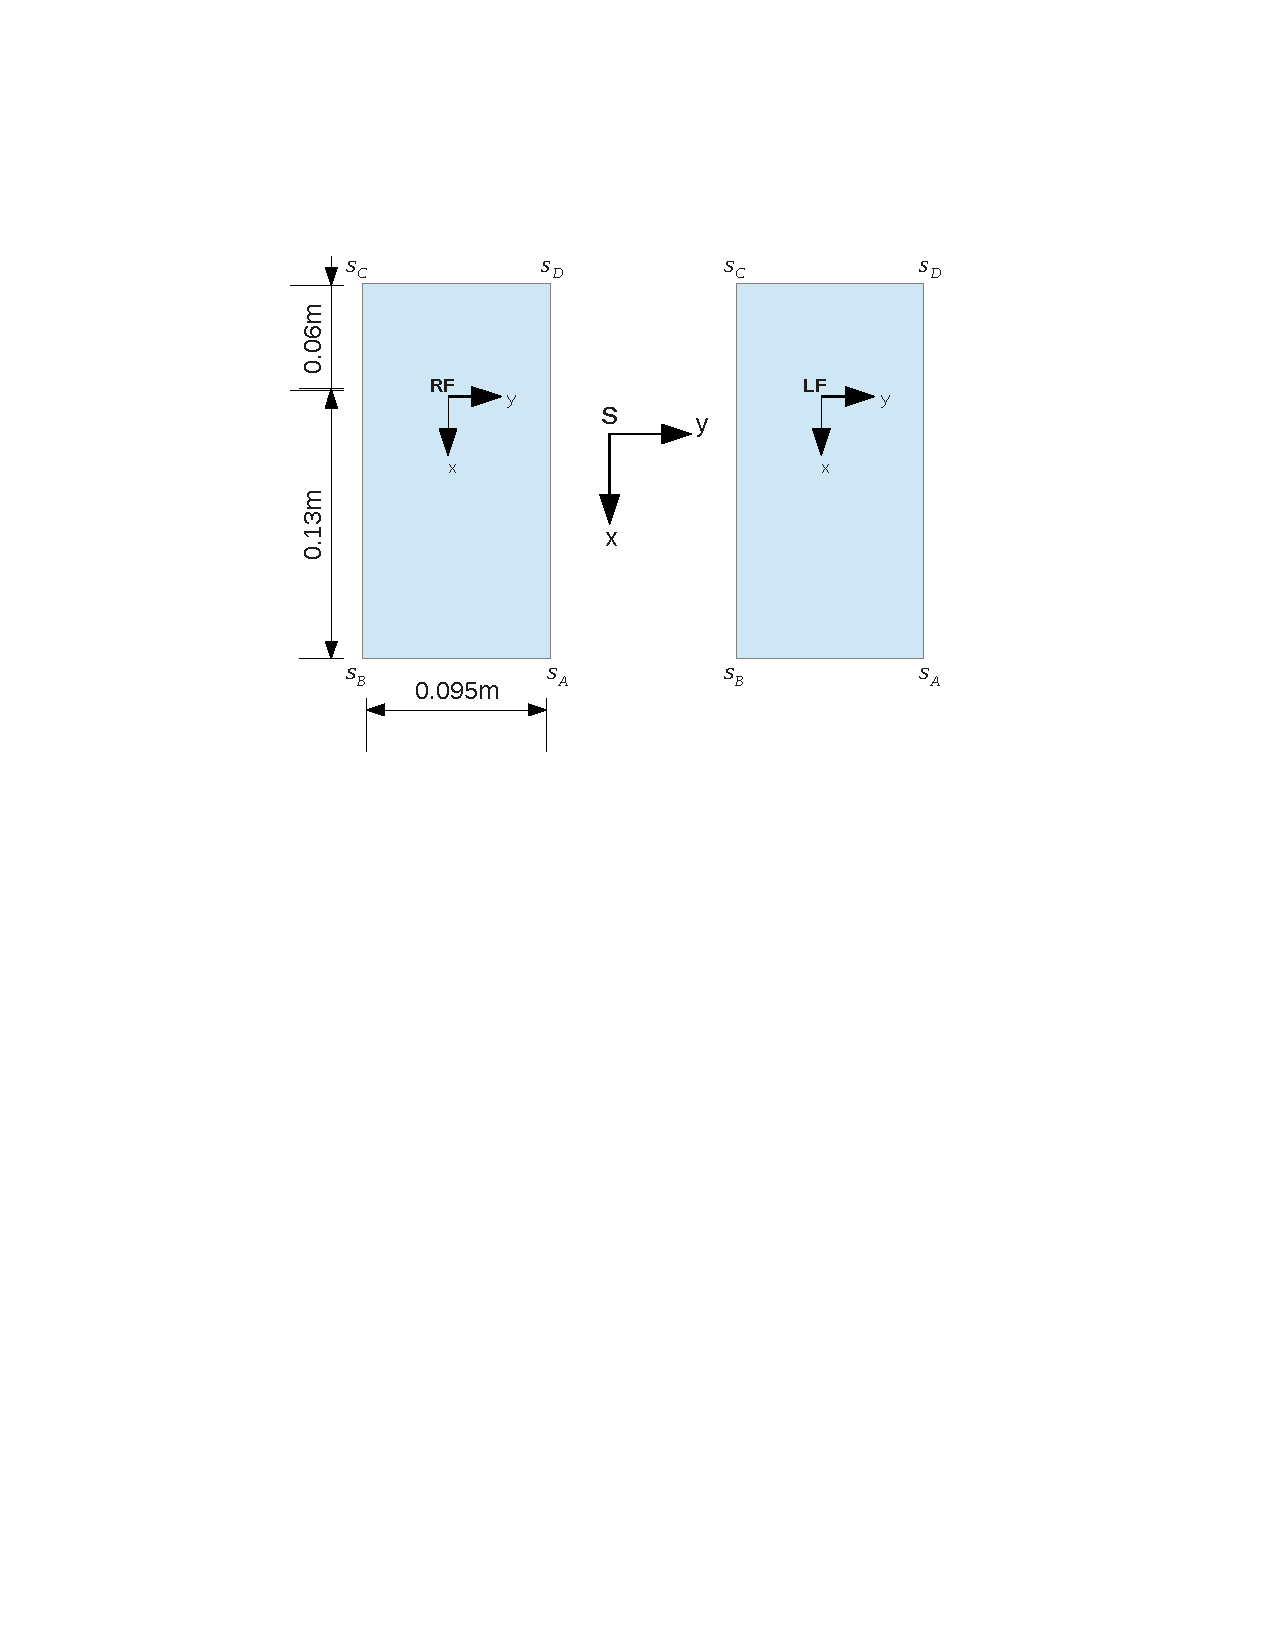
\includegraphics[trim= 20mm 150mm 20mm 50mm,scale=0.80]{Bilder/foot_topview.pdf}
    \caption{Toro feet viewed from top}
    \label{fig:biped_feet}
    \end{center}
\end{figure}
Along with the sensor measurements kinematic constraints are also considered as mesurement. When a foot is in contact with the ground the velocity of the foot is zero. Figure \ref{fig:biped_feet} shows the contact points considered for measurements. The corner points of each foot are measured with respect to spatial frame \emph{S} as shown in Figure \ref{fig:biped_feet} before starting the experiment and they are assumed to be constant throughout the experiment. The contact points of the robot does not change throughout the experiment, since we are considering the case where the robot is tilting around one edge of the foot. 
<<<<<<< HEAD
=======
\begin{equation}
    \begin{split}
    y_{kin} &=
    \begin{bmatrix}
    p_{contact} \\ V_{contact}
    \end{bmatrix}\\
    p_{contact} &= \begin{bmatrix}p_{RF}\\ p_{LF}\end{bmatrix}\\
     V_{contact} &= \begin{bmatrix} V_{RF}^b \\ V_{LF}^b \end{bmatrix} = \begin{bmatrix} J_r(y)^T \dot{q} \\ J_l(y)^T\dot{q} \end{bmatrix}
    \end{split}
\end{equation}
\begin{itemize}
\item $p_{RF},p_{LF}$ are the vectors of contact points in right foot and left foot defined with respect to spatial frame.
\item $J_r(y), J_l(y)$ are the Jacobians of right and left foot that relates the joint velocity to the velocity of right and left foot respectively. \underline{[Appendix Define Body Jacobian]}
\end{itemize}
\begin{equation}
    \begin{split}
    p_{RF} &= \begin{bmatrix} p_{A,RF}\\ p_{B,RF}\\ p_{C,RF}\\ p_{D,RF}\end{bmatrix}= \begin{bmatrix} H_{RF}p_{A}\\  H_{RF}p_{B}\\  H_{RF}p_{C}\\  H_{RF}p_{D}\end{bmatrix} \\
    p_{LF} &= \begin{bmatrix} p_{A,LF}\\ p_{B,LF}\\ p_{C,LF}\\ p_{D,LF}\end{bmatrix}= \begin{bmatrix} H_{LF}p_{A}\\  H_{LF}p_{B}\\  H_{LF}p_{C}\\  H_{LF}p_{D}\end{bmatrix} \\
    \end{split}
\end{equation}
\begin{itemize}
\item $H_{RF},H_{LF}$ are the homogeneous transformation matrices of the right and left foot.\underline{Appendix Homogeneous Transformation Matrix}
\end{itemize}
\begin{comment}
\item $\omega_{f}^{b} $ is the vector of angular rates of floating base in body frame (measured by Gyroscope). 
\item $\ddot{p}_{f}^{b}$ is the vector of Cartesian accelerations of the floating base in body frame (measured by IMU).	$\ddot{q}(1,2,3)$ is the first three elements of $\ddot{q}$ computed by Eq. \ref{eq:motion}. $R_{sb}^{T}(0,0,9.81)^{T}$ is the term added to compensate for the gravity measured by IMU. 
\item $p_{c}^{b}$ is the vector of position constraints of right and left foot. These positions constraints are the static points on the foot of the robot. $H_{sx}$ is the homogeneous transformation matrix from frame \emph{x} to spatial frame. $p_{a,r}^{s}, p_{b,r}^{s}, p_{a,l}^{s}, p_{b,l}^{s}$ are known points which are constant with respect to spatial frame.
\item $\hat{V}_{c}^{b}$ are velocity constraints on right and left foot.

\end{comment}

For computation of measurement matrix \emph{C} the derivative of y in Eq. \ref{eq:toro} with respect to system state is computed.
>>>>>>> 44a31b53d04194cb885ea2522465b774c238d9f2
\begin{equation}
    \label{eq:y_kin}
    \begin{split}
    y_{kin} &=
    \begin{bmatrix}
    p_{contact} \\ V_{contact}
    \end{bmatrix}\\
    p_{contact} &= \begin{bmatrix}p_{RF}\\ p_{LF}\end{bmatrix}\\
     V_{contact} &= \begin{bmatrix} V_{RF}^b \\ V_{LF}^b \end{bmatrix} = \begin{bmatrix} J_r(\hat{y})^T \hat{\dot{q}} \\ J_l(\hat{y})^T\hat{\dot{q}} \end{bmatrix}
    \end{split}
\end{equation}
\begin{itemize}
\item $p_{RF},p_{LF}$ are the vectors of contact points in right foot and left foot defined with respect to spatial frame.
\item $J_r(y), J_l(y)$ are the Jacobians of right and left foot that relates the joint velocity to the velocity of right and left foot respectively. \underline{[Appendix Define Body Jacobian]}
\end{itemize}
\begin{equation}
    \begin{split}
    p_{RF} &= \begin{bmatrix} p_{A,RF}\\ p_{B,RF}\\ p_{C,RF}\\ p_{D,RF}\end{bmatrix}= \begin{bmatrix} {H}_{RF}p_{A}\\  {H}_{RF}p_{B}\\  {H}_{RF}p_{C}\\  {H}_{RF}p_{D}\end{bmatrix} \\
    p_{LF} &= \begin{bmatrix} p_{A,LF}\\ p_{B,LF}\\ p_{C,LF}\\ p_{D,LF}\end{bmatrix}= \begin{bmatrix} {H}_{LF}p_{A}\\  {H}_{LF}p_{B}\\  {H}_{LF}p_{C}\\  {H}_{LF}p_{D}\end{bmatrix} \\
    \end{split}
\end{equation}
\begin{itemize}
\item $\hat{H}_{RF},\hat{H}_{LF}$ are the homogeneous transformation matrices of the right and left foot.\underline{Appendix Homogeneous Transformation Matrix}
\item In Figure \ref{fig:biped_feet} $p_A,p_B,p_C,p_D$ are the corner points defined with respect to respective foot frame \emph{RF,LF}.
\end{itemize}
The full measurement equations of is obtained combining Equations \ref{eq:y_sens} and \ref{eq:y_kin} 
\begin{equation}
    \label{eq:y_msr}
    y_{k+1} = \begin{bmatrix} y_{sens,k+1} \\ y_{kin,k+1} \end{bmatrix}
\end{equation}
The measurement sensititvity matrix can be computed by taking the parial derivative of the mesaurement equation \ref{eq:y_msr} with respect to system states \emph{x}.
\begin{enumerate}
\item $\hat{acc}^b_{k+1} = \ddot{p}_{k+1}-\hat{R}^T\begin{bmatrix} 0 \\ 0 \\ -9,81 \end{bmatrix}$
\begin{equation}
    \label{eq:dacc_msrdx}
    \dfdx{\hat{acc}_{k+1}^b}{x} = \dfdx{\hat{\ddot{p}}_{k+1}^b}{x} + \dfdx{\hat{R}^T_{k+1}}{x}\begin{bmatrix} 0 \\ 0 \\ -9,81 \end{bmatrix}  \in \Re^{3 \times 62}
\end{equation}
\begin{itemize}
    \item $\dfdx{\hat{\ddot{p}}_{k+1}^b}{x}$ is parital derivative of acceleration of body with respect to states of the system. It is computed by substituting $\hat{x}_{k+1}^-$ for $\hat{x}_k$ in Equation \ref{eq:dydx} and then subtracting  $l_{31,i-31}$ for the case \emph{i > 31}. The first three rows of the reuslting matrix is the partial derivative of acceleration with respect to states.
    \item $\dfdx{\hat{R}^T_{k+1}}{x}$ is partial derivative of Rotation matrix with respect to system state.[Appendix \ref{sec:rot_mat}]
\end{itemize}

\item $\hat{\omega}^{b-}_{k+1}$
\begin{equation}
    \label{eq:dw_msrdx} 
    \dfdx{\hat{\omega}^{b-}_{k+1}}{x} = \left(\dfdx{\hat{\omega}^{b-}_{k+1}}{x_{1}}, \dfdx{\hat{\omega}^{b-}_{k+1}}{x_{2}}, \cdots , \dfdx{\hat{\omega}^{b-}_{k+1}}{x_{62}}\right) \in \Re^{3 \times 62}
\end{equation}
\[ \dfdx{\hat{\omega}^{b-}_{k+1}}{x} = 
    \begin{cases}
    l_{3,34-i} & \text{if } 34 < i \leq 37 \\
    \textbf{0}_{3,1} &\text{otherwise}
    \end{cases}
 \]  
 
\item $\hat{q}_{k+1}^-$
\begin{equation}
\label{eq:dq_msrdx}
\dfdx{\hat{q}_{k+1}^-}{x} = \left(\dfdx{\hat{q}_{k+1}^-}{x_{1}}, \dfdx{\hat{q}_{k+1}^-}{x_{2}}, \cdots , \dfdx{\hat{q}_{k+1}^-}{x_{62}}\right) \in \Re^{25 \times 62}
\end{equation}
 \[
 \dfdx{\hat{q}_{k+1}^-}{x_{i}} =
 \begin{cases}
 1 & \text{if } 7 \leq i \leq 31 \\
 0 & \text{otherwise}
 \end{cases}
 \]

\item  $\hat{\dot{q}}_{k+1}^-$
\begin{equation}
 \label{eq:ddq_msrdx}
\dfdx{\hat{\dot{q}}_{k+1}^-}{x} = \left(\dfdx{\hat{\dot{q}}_{k+1}^-}{x_{1}}, \dfdx{\hat{\dot{q}}_{k+1}^-}{x_{2}}, \cdots , \dfdx{\hat{\dot{q}}_{k+1}^-}{x_{62}}\right) \in \Re^{25 \times 62}
\end{equation}
  \[
 \dfdx{\hat{\dot{q}}_{k+1}^-}{x_{i}} =
 \begin{cases}
 1 & \text{if } 37 < i \leq 62 \\
 0 & \text{otherwise}
 \end{cases}
 \]
 
\end{enumerate}
\begin{equation}
\label{eq:dmsr_dpc}
\dfdx{p_{c}^{b}}{x} = \left(\dfdx{p_{c}^{b}}{x_{1}}, \dfdx{p_{c}^{b}}{x_{2}}, \cdots , \dfdx{p_{c}^{b}}{x_{62}}\right) \in \Re^{12 \times 62}
\end{equation}
\[
\dfdx{p_{c}^{b}}{x_{i}} =
\begin{cases}
\left(
\begin{aligned}
-H_{sr}^{-1}\dfdx{H_{sr}}{x_{i}}H_{sr}^{-1}p_{a,r}^{s} \\
-H_{sr}^{-1}\dfdx{H_{sr}}{x_{i}}H_{sr}^{-1}p_{b,r}^{s} \\
-H_{sl}^{-1}\dfdx{H_{sl}}{x_{i}}H_{sl}^{-1}p_{a,l}^{s} \\
-H_{sl}^{-1}\dfdx{H_{sl}}{x_{i}}H_{sl}^{-1}p_{b,l}^{s}
\end{aligned} \right)
& \text{if } 1 \leq i \leq 31 \\
0 &\text{otherwise}
\end{cases}
\]
 \begin{equation}
 \label{eq:dmsr_dvc}
\dfdx{\hat{V}_{c}^{b}}{x} = \left(\dfdx{\hat{V}_{c}^{b}}{x_{1}}, \dfdx{\hat{V}_{c}^{b}}{x_{2}}, \cdots , \dfdx{\hat{V}_{c}^{b}}{x_{62}}\right) \in \Re^{12 \times 62}
\end{equation}
\[
\dfdx{\hat{V}_{c}^{b}}{x_{i}} = 
	\begin{cases}
	\left(
	\begin{aligned}
	\dfdx{J_{r}^{b}}{x_{i}}\dot{q} \\
	\dfdx{J_{l}^{b}}{x_{i}}\dot{q} \\
	\end{aligned} \right)
	& \text{if } 1 \leq i \leq 31 \\
	\begin{pmatrix}
	col(J_{r}^{b},i)\\ col(J_{l}^{b},i)
	\end{pmatrix}
	 	& \text{if } 32 \leq i \leq 62
	\end{cases}
\]
The measurement matrix of the system is given by Eq. \ref{eq:dmsr_q}, \ref{eq:dmsr_dq}, \ref{eq:dmsr_dacc}, \ref{eq:dmsr_dtheta}, \ref{eq:dmsr_dpc}, \ref{eq:dmsr_dvc}
\begin{equation}
C = \left(
   \begin{aligned}
   \dfdx{q}{x} \\
	 \dfdx{\dot{q}}{x}\\
	 \dfdx{\ddot{p}_{f}^{b}}{x}\\
	 \dfdx{\dot{\theta}_{f}^{b}}{x}\\
	 \dfdx{p_{c}^{b}}{x}\\
	 \dfdx{\hat{V}_{c}^{b}}{x} 
   \end{aligned}
	 \right) \in \Re^{80 \times 62}
\end{equation}

\begin{comment}
This is a code to format lengthy equations.
\[
  \text{left hand side} =
  \begin{cases}
    \!\begin{aligned}%[b]
       & \text{a very long expression} \\
       & + \text{that continues on the next line}
    \end{aligned}           & \text{1st condition} \\%[1ex]
    \text{short expression} & \text{2nd condition}
  \end{cases}
\]
\end{comment}
\end{enumerate}
\paragraph{Observability:}
State space representation of a linear system is,
\begin{equation}
\label{eq:dyn_l}
\begin{split}
\dot{x} &= Ax + Bu\\
y &= Cx + Du.
\end{split}
\end{equation}
where, $x \in \Re^{n}$ is the vector representing the states of the system. $u \in \Re^{p}$ is the vector of inputs, $y \in \Re^{m}$ is the vector of outputs of the system. $A \in \Re^{n \times n}$ is the system matrix. $B \in \Re^{n \times p}$ is the matrix relating state and input, $C \in \Re^{m \times n}$ is the measurement matrix relating output and state, $D \in \Re^{m \times p}$ is the matrix relating input and output of the system.

Linearising a non linear system in Equation \ref{eqn:nl_sys} at some operating point will lead to linear system of form Eq. \ref{eq:dyn_l}. For a linear system to be observable, it should satisfy
\begin{equation}
obs =
\begin{pmatrix}
C\\ CA \\ CA^{2}\\ \vdots \\ CA^{n-1}
\end{pmatrix}
, rank(obs) =n
\end{equation}
For our system to be observable $rank(obs) = 62$.
<<<<<<< HEAD

\textbf{ Make plots from files act=datsrc/ROBOT-TILT-0807.mat est=estimates-data/est-090701.mat or *080703.mat }
=======
	
>>>>>>> 44a31b53d04194cb885ea2522465b774c238d9f2
%\end{document}
